\title{EN.601.448/648 Computational genomics: \\
Final Project - Midterm report}
\author{
        {Ayush Agarwal (aagarw33)}  \\
                Computer Science (Masters)\\
            \and
        {Lohita Sivaprakasam (lsivapr1)}  \\
                Computer Science (Masters)\\
                \and
        {Satish Palaniappan (spalani2)}  \\
                Computer Science (Masters)\\
                \and
        {Srivathsa Pasumarthi (psrivat1)}  \\
                Computer Science (Masters)\\
}
\date{\today}

\documentclass[12pt]{article}
\usepackage{graphicx}
\usepackage{wrapfig}
\usepackage{url}
\usepackage{wrapfig}
\usepackage{color}
\usepackage{marvosym}
\usepackage{enumerate}
\usepackage{subfigure}
\usepackage{tikz}
\usepackage[fleqn]{amsmath}
\usepackage{amssymb}
\usepackage{hyperref}
\usepackage[many]{tcolorbox}
\usepackage{lipsum}
\usepackage{float}
\usepackage{trimclip}
\usepackage{listings}
\usepackage{environ}% http://ctan.org/pkg/environ
\usepackage{wasysym}
\usepackage{array}
\usepackage[margin=1in]{geometry}
\usepackage{multirow}


\begin{document}
\maketitle

Due: 4/12/2019

\section{Problem}
In this project, our primary aim is to perform taxonomic-classification of bacterial DNA
using various machine learning and deep learning approaches. The DNA sequences for these single-cell microorganisms serve as a unique identifier (like a barcode) for that species and characterizes each of them completely. Following \cite{src_work} as the base literature, we would like to perform the same classification using various other machine learning and deep learning approaches as described below and compare each method using defined metrics. Secondly, we would also like to use deep representation learning approaches to model meaningful representations of the DNA sequences and use these representations to perform hierarchical agglomerative clustering to validate if they correlate with their actual taxonomic hierarchy.

\section{Data}
We are using the same data as of \cite{src_work} which is from the Ribosomal Database Project (RDP \cite{rdp} -
{\color{blue}\href{https://rdp.cme.msu.edu/download/current_Bacteria_unaligned.fa.gz}{Download Link}}) and consists of around $\sim$550K samples of bacterial DNA along with the information about its taxa - phylum, class, order, family, genus. The source FASTA file was processed and samples whose sequence lengths were between 400 and 440 were picked; this choice was made only for keeping the sequence lengths almost constant while maximizing the total number of samples. The final data consists of $\sim$9174 samples spanning over 3 phyla, 5 classes and 19 orders.
\\
\\
In order to tackle the extreme imbalance in the \textit{order} level, we have grouped the samples that are under-represented, into a single class named \textit{Others}. The \textbf{train-test-validation split is 60\%, 20\% and 20\%} respectively. The choice of dataset split was intuitive as we wanted to give enough samples for parameter tuning and validation, given the relatively small number of samples.
\\
\\
Instead of doing multi-category classification, we are solving three separate classification problems by generating separate data files for phylum, class and order; this is a conscious choice in order tackle the problem of class imbalance in the lower levels of the hierarchy and to avoid multiplicative error transmission from top to bottom in the hierarchy.

\section{Methods}
    \subsection{Methods for Taxonomic-Classification}
        \subsubsection{General Machine Learning methods (Features: k-mer counts)}
        Normalized k-mer counts were extracted from the dataset and stored as individual feature matrices for different K values. Using these features, SVM and Random Forest models were trained for classifying the phylum, class and order. The goal here is to find the ideal K value that represents the data with the right amount of context, using the basic ML methods. F1 scores were calculated for the different models separately, for each K value ranging from 3 to 6. SVM and Random Forest both perform almost equally well with an average F1 score of 0.94. Detailed analysis of results can be found in Section 5.1

        \subsubsection{General Machine Learning methods (Features: vector representation)}

        Another type of encoding used was the ordinal encoding of the gene data where each of the four types (A, C, G, T) and an additional type (to accommodate all other data apart from the above), were encoded as separate real number representations. This was constructed as a direct mapping and each sample's sequence was simply converted to a vector-based representation of the same length. Using these features, SVM and Random Forest classifiers were trained for the phylum and class level hierarchy. This method was directly compared to the previously explained k-mer based encoding method, to understand the importance of sequence encodings in our dataset. An average F1 score of about 0.79 was obtained for the phylum classification using both the models.

        \subsubsection{Convolutional Neural Networks (Features: QRCode-like image representation of DNA sequences)} \label{cnn}
        Here we would like to explore an interesting way to represent a DNA sequence, which would be to visualize them as QRCode-like images. An example of how this encoding technique works is shown in Figure \ref{fig:qrcode}. As the sequences in the dataset are of varying length, we first take the length of the longest sequence and ceil its square root and take this number, D, as the max width and height of the image to be generated. Then we take each sequence in the dataset and reshape them to $D * D$, 2D arrays, by padding the 2D array with zeros where there is no information. Then we one-hot encode each cell based on the A, C, G, T base pairs, thus leading to an array of size  $D * D * 4$, where 4 is the number of channels of the image. Just for the sake of visualizing this as an image, we assigned 4 colours namely Red, Green, Blue and Orange for A, C, G, and T respectively (and black for no information). For our dataset here with N samples, as the maximum sequence length is 440bp, we generate a dataset of dimensions $N * 21 * 21 * 4$.

        These DNA QRCodes were then used as the input features for training the Convolutional Neural Network who's architecture is as defined in Figure \ref{fig:cnnarch}. This network was trained using a Negative Log-likelihood loss which was optimized using the Adam optimizer with a learning rate of $0.001$ for $25$ epochs with a batch size of $32$.

        \begin{figure}[h]
        \centering
        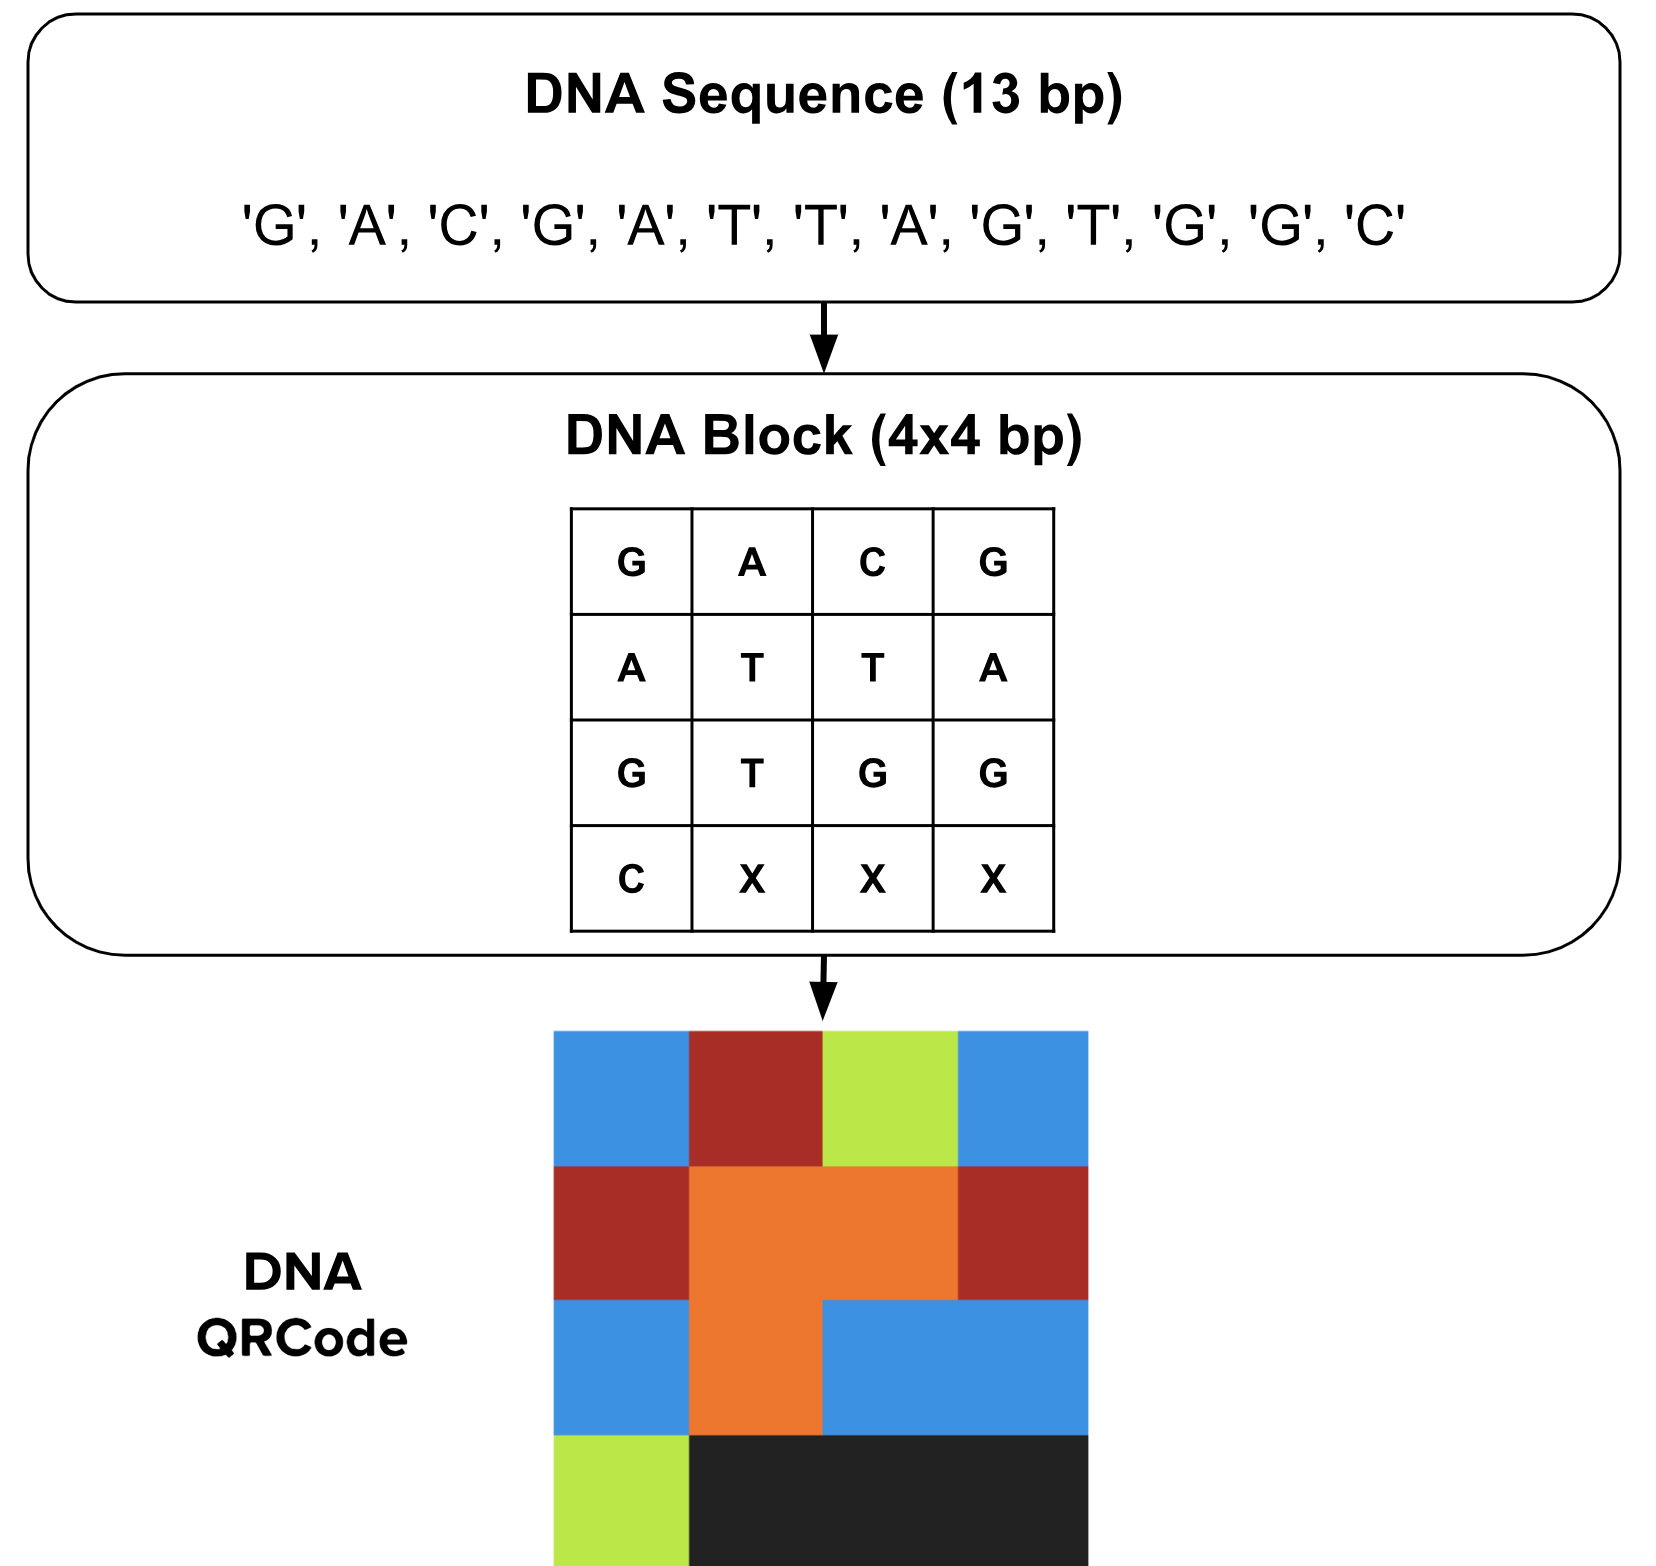
\includegraphics[scale=0.3]{QRCode.png}
        \caption{QR-code like DNA sequence representation}
        \label{fig:qrcode}
        \end{figure}

        \begin{figure}[h]
        \centering
        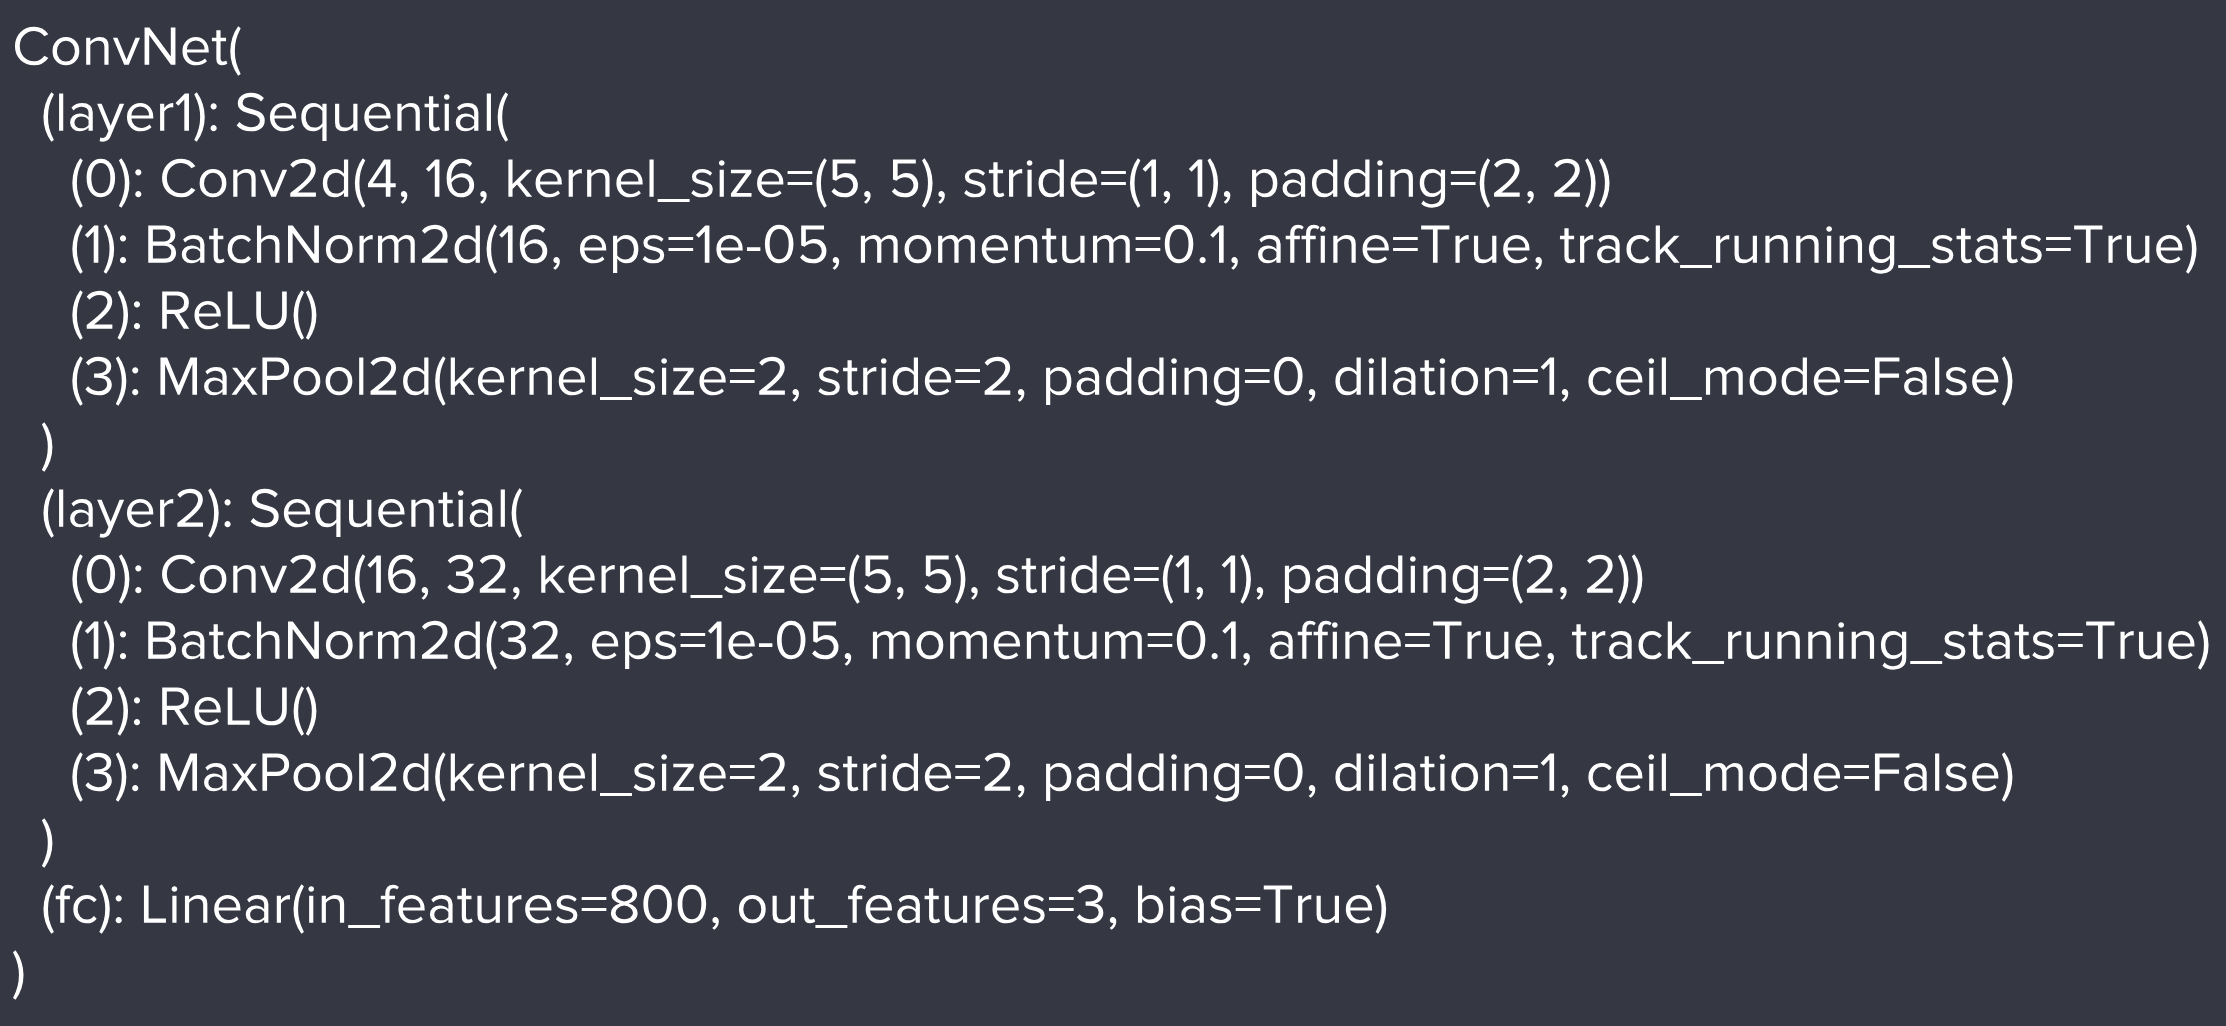
\includegraphics[scale=0.3]{cnn_arch.png}
        \caption{CNN Architecture}
        \label{fig:cnnarch}
        \end{figure}

        \subsubsection{Recurrent Neural Networks - LSTM (Features: Raw DNA sequences)}
        \label{subsection: rnn}
        Given the lack of explicit features and high dimensionality of the DNA sequences, recurrent neural networks(RNNs) provide an efficient way to encode the sequences for classification. Long Short Term Memory(LSTM) is a special type of RNNs, which is also composed of a chain of repeating modules of neural networks. Contrary to the standard RNNs that have a single tanh layer as the repeating module, LSTMs have four layers that interact with each other in order to handle the long-range dependencies with the aid of input, forget and output gates. In this approach, we are making use of LSTM networks due to their ability to process entire sequences and preserve the entire sequence's information irrespective of the gap length in huge sequences.

        We have carried out experiments with the raw DNA sequences as the input to the LSTM and attempted to classify the sequences with respect to their phylum, class and order labels. The LSTM network was trained to closely predict the ground truth labels, by means of optimizing the negative log-likelihood loss with an Adam optimizer at a learning rate of 0.001. The obtained results and their analysis are presented in Section \ref{subsection: rnnresults}.


        \subsection{Representation Learning and Agglomerative Clustering}
        Deep representation learning has been used in recent years for various applications such as clustering, classification and data compression. Our goal here is to apply various representation learning techniques such as Variational Auto-Encoders (VAE) and LSTM Auto-Encoders to learn a representation of the DNA sequence and use that representation as features to perform hierarchical agglomerative clustering. The clustering is done to verify and validate that the learned representations actually correlate with their taxonomic hierarchy.


    \subsection{Ambitious Goals}
        These tasks will be done based on the availability of time and resources.

        \subsubsection{Ensemble Learning}
        We will attempt to learn multiple possibly uncorrelated learners to solve the same problem with sub-sampled data and combine these models to learn a meta-learner using stacking techniques such as an MLP, to get a much improved final prediction accuracy. This will help us leverage the advantages of multiple machine learning models.

        \subsubsection{Hybrid CNN-RNN approach}
        Here we borrow one of the key ideas from deep-learnt image captioning architectures which use both CNNs and RNNs to learn representations of data and combine them into a richer lower dimension space to get a hybrid data representation that facilitates feature interaction among different types of data. Using this as key, we combine the QRCode-like representation of a DNA sequence run over a CNN and the raw DNA sequence run over an RNN using fully connected layers to finally perform taxonomy-classification, which we believe will give better results.

        \subsubsection{Family Level Classification}
        When we move to the family level of the hierarchy, the dataset we have suffers from very high class-imbalance and with a high number of classes to predict as well. In order to train models in spite of this, we propose to group the classes with an almost same number of samples in a single dataset and produce N such datasets. Then we can train N different ML models on these datasets and bag their results to predict the final label, and if we are using Deep-learnt models like a CNN or RNN, we can use weighted loss functions to account for the class imbalance, where the weights are determined by the class imbalance proportions.

\section{Evaluation metrics}
We would like to use the following metrics used to evaluate any standard supervised classification or unsupervised clustering problem:
\begin{enumerate}
    \item \textbf{Classification Problem:} Overall accuracy, Per category accuracy, False Positive Rate, F1 score (Good metric for classification as it is the harmonic combination of precision and recall) and weighted F1 and Accuracy scores.
    \item \textbf{Clustering Problem:} Mutual Information Score, Homogeneity Score
\end{enumerate}

\section{Results}
        \subsection{General Machine Learning methods (Features: k-mer counts)}
        Figure \ref{fig:svm_kmer} and Figure \ref{fig:rf_kmer} shows the K-mer wise F1 score counts. We observe that Random Forest classifier performs slightly better, but the peak is at k=5 for both classifiers. From these figures, we can infer that k=5 is an ideal setting in terms of the context in the DNA sequence that it provides and also in the number of features ($4^5$) which is not too little nor too much. Hence 5-mers represent the data precisely which 3-mers and 4-mers do not do due to both the lack of context and lack of number-of-features. There is a significant drop in F1 score for k=6 because, at this point, the number of features ($4^6$) becomes greater than the number of samples.

        \begin{figure}[h]
        \centering
        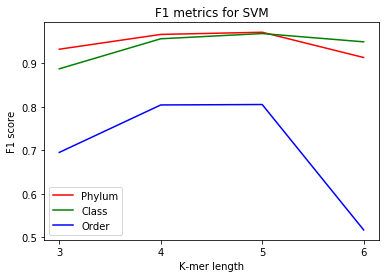
\includegraphics[scale=0.5]{svm_kmer}
        \caption{K-mer wise F1 scores for SVM}
        \label{fig:svm_kmer}
        \end{figure}

        \begin{figure}[h]
        \centering
        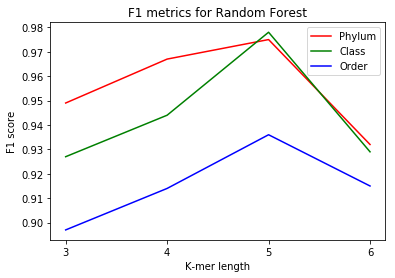
\includegraphics[scale=0.5]{rf_kmer}
        \caption{K-mer wise F1 scores for Random Forest classifier}
        \label{fig:rf_kmer}
        \end{figure}

        \subsection{General Machine Learning methods (Features: vector representation)}
        The results obtained for the phylum classification were encouraging, with the simple encoding, leading to validation and test accuracies close to 88\% for the random classifier and about 81\% for SVM. The ROC curve for the same is as seen in Figure \ref{fig:svm_vec}.

        \begin{figure}[h]
        \centering
        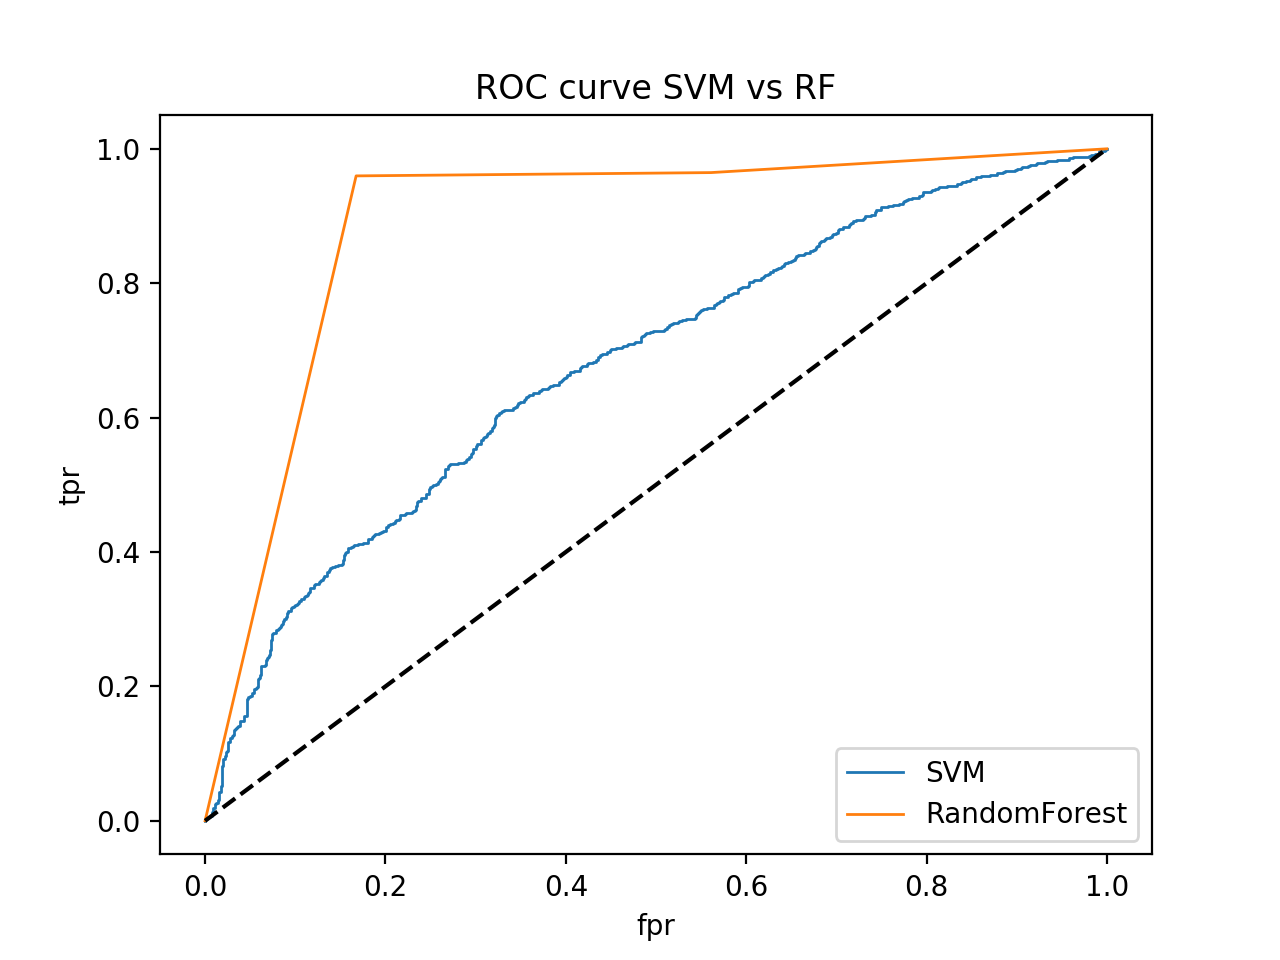
\includegraphics[scale=0.5]{roc_phylumpng.png}
        \caption{ROC curves for phylum classification - vector encoding}
        \label{fig:svm_vec}
        \end{figure}

        \begin{figure}[h]
        \centering
        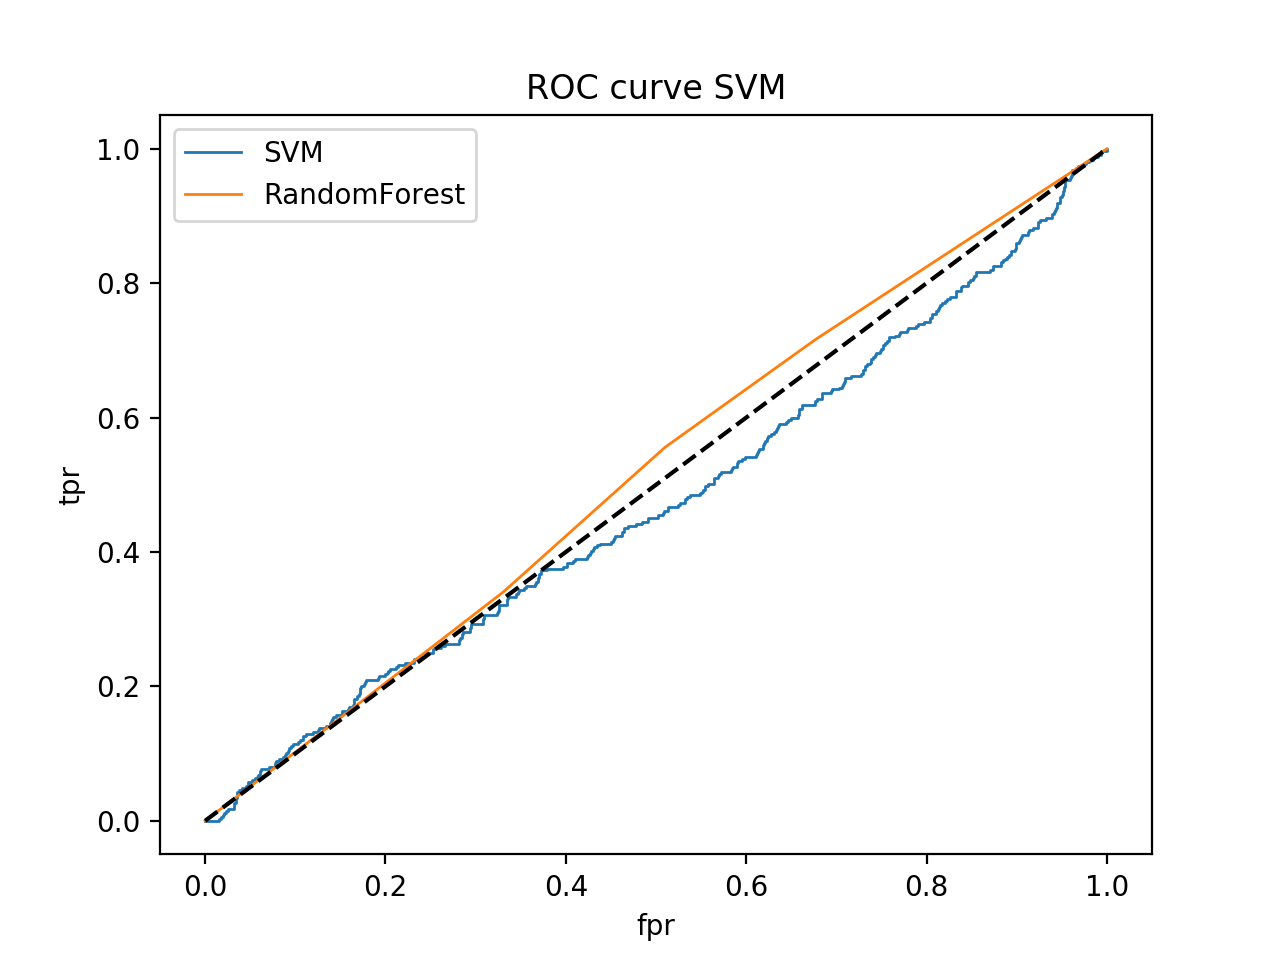
\includegraphics[scale=0.5]{svmrf_roc.png}
        \caption{ROC curves for Class classification - vector encoding}
        \label{fig:class_svm}
        \end{figure}

        When the confusion matrix for the above classification was extracted, it was found that most errors lay in false positives, appearing where the positive class was the most dominant class in terms of samples. Although the skew in phylum classes is less, the above property indicates that classification on the basis of Class and Order may not perform well for the given encoding method.

        As a next step, the same methods were applied to the Class level classification to test the previous hypothesis. As expected, poor results were obtained with F1 scores using both Random Forest and SVM, languishing at 20\% and according to the confusion matrix, it was observed that most prediction allotments were done towards the class having the most number of samples. The ROC curve for the same can be seen in Figure \ref{fig:class_svm}.
        \newline
        Order level classification gave an even worse performance having an F1 score of 15\% on the 10 order classes.

        \subsection{Convolutional Neural Networks (Features: QRCode-like image representation of DNA sequences)}
        We train the Convolutional Neural Network on the DNA QRCodes as described in Section \ref{cnn}. We repeat the training for each level of the taxonomy hierarchy, namely Phylum, Class and Order. We train on the training dataset and evaluate on the test dataset, but for time being we haven't used the validation dataset to optimize over the CNN parameters, which we will do later. The test accuracy of the Phylum, Class and Order classifiers are 99.29\%, 98.85\% and 93.57\% respectively, and the accuracy vs epochs plot can be found in Figure \ref{fig:cnnacc}. To see more plots, visualizations and results, have a look at the Jupyter Notebook hosted {\color{blue}\href{https://nbviewer.jupyter.org/urls/dl.dropbox.com/s/ynwxw8pd82x1mi2/CNN\%20-\%20DNA\%20QRCode\%20Based.ipynb}{here}}.
        \newline
        From the accuracy plots it is also evident that the \textbf{CNN model as described in Figure \ref{fig:cnnarch} trained on the DNA QRCodes majorly outperforms all the models and methods we have experimented with}, including SVMs, Random Forests, and RNNs, by achieving the highest accuracy possible for each of the three levels of classification tasks. Other inferences from the accuracy plots are that the Phylum and Class models are well trained and do not suffer from the overfitting problem and generalize well to unseen samples, while the Order level CNN model, actually starts to slightly overfit the data and hence the gap between the train and test accuracy curves. Which can be alleviated by introducing regularization techniques like dropouts and L2 weight decay, which we will try out and report in our final proposal.

        \begin{figure}[h]
        \centering
        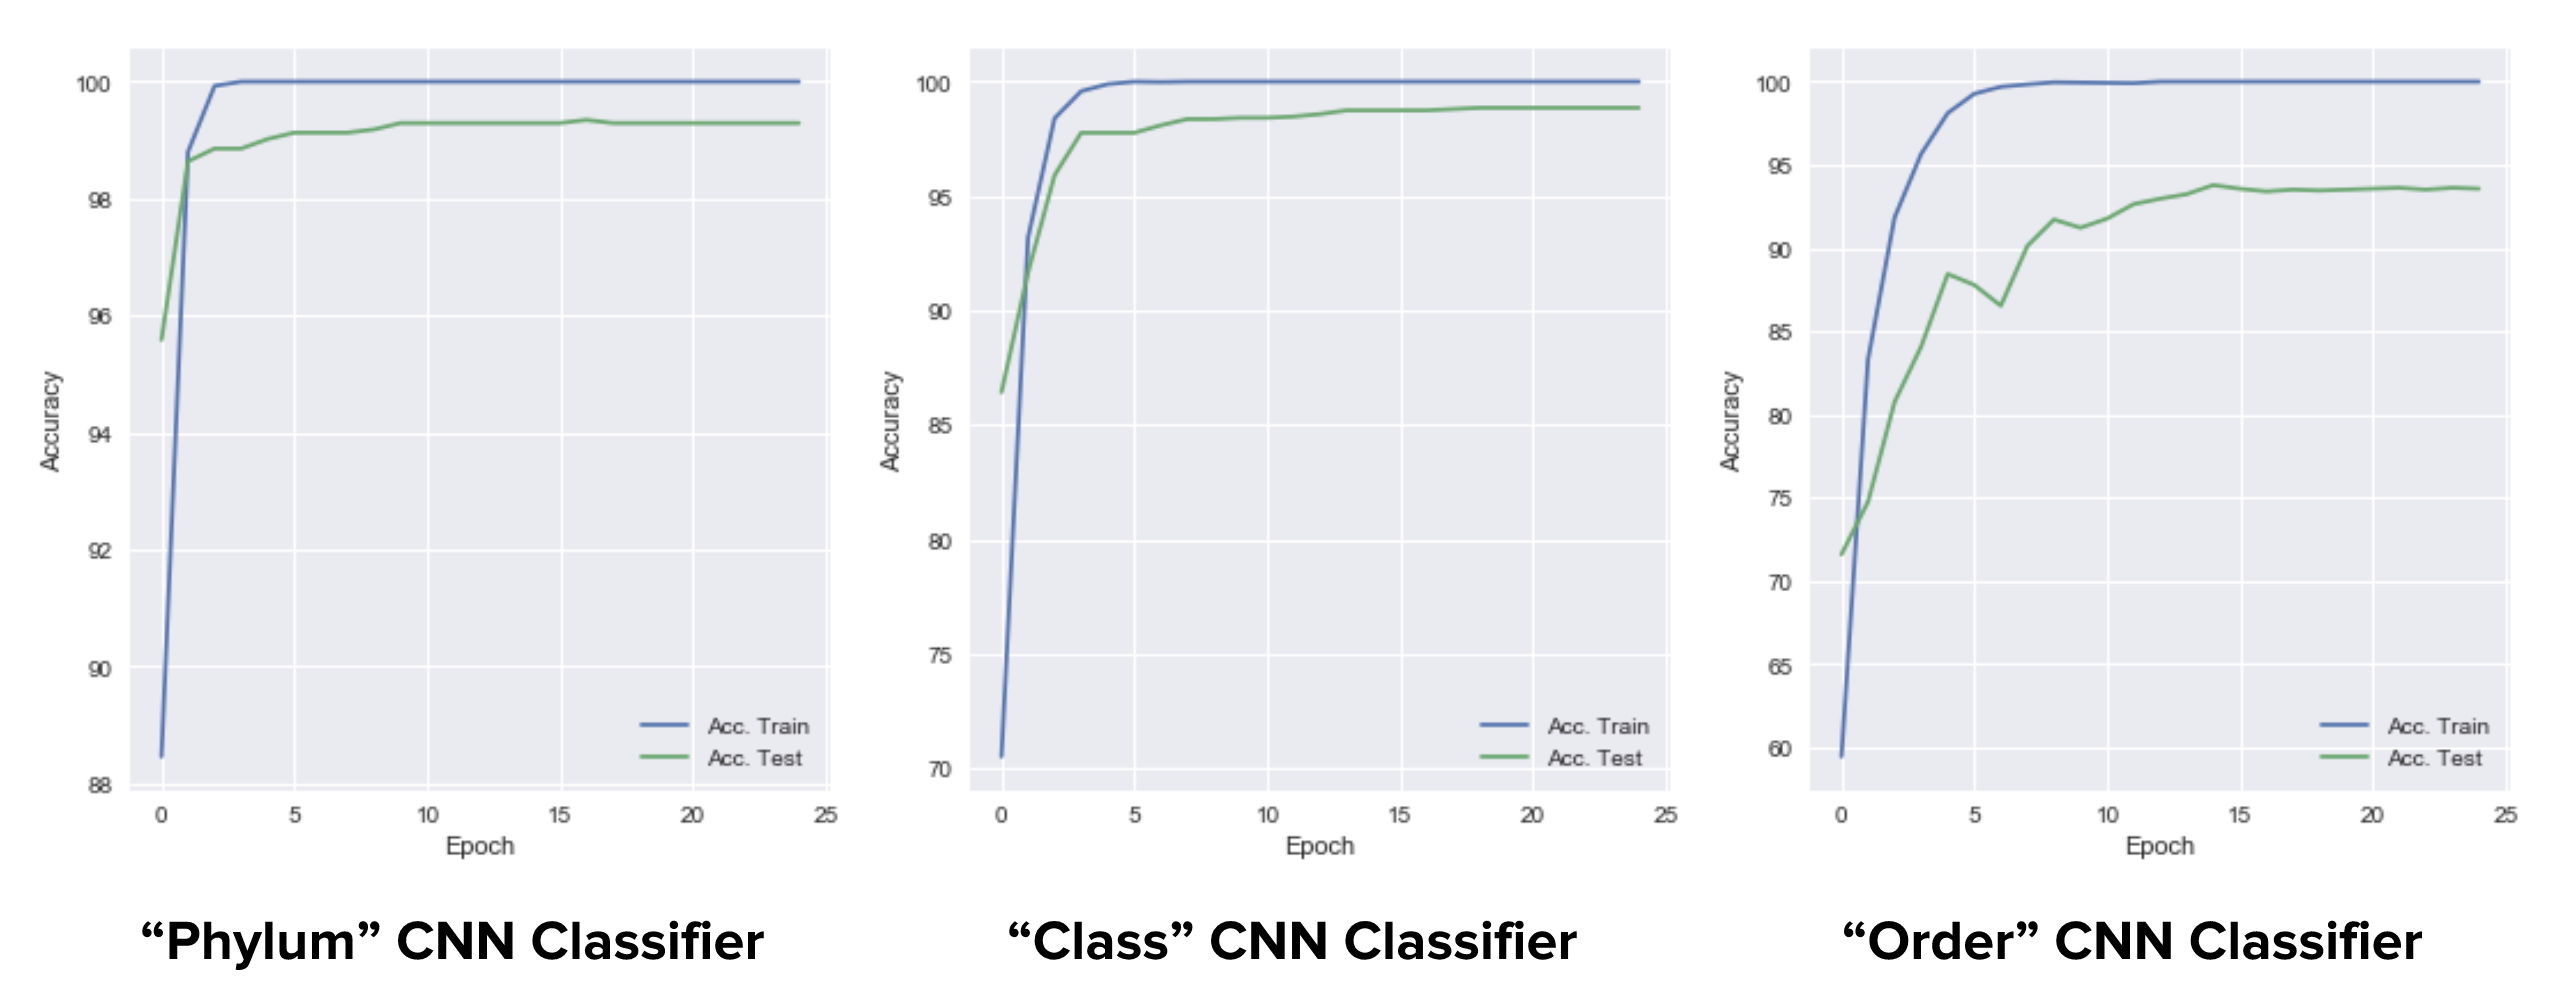
\includegraphics[scale=0.35]{cnn_acc_plots.png}
        \caption{Accuracy vs Epochs Plot: CNN (QRCode)}
        \label{fig:cnnacc}
        \end{figure}

        \subsection{Recurrent Neural Networks - LSTM (Features: Raw DNA sequences)}
        \label{subsection: rnnresults}
        As stated in Section \ref{subsection: rnn}, we have attempted to classify the LSTM encoded DNA sequences based on three different levels, namely phylum, class and order. This approach gives us an insight into the degree to which the LSTM encoded DNA sequences are indicative of the phylum, class and order to which they belong. The F1 scores obtained on each of the classification tasks are presented in Table \ref{table:lstmeval} below. The test accuracies for Phylum, Class and Order classifiers are 97.6\%, 94.7\% and 89.1\% respectively. The F1 scores measured are the weighted F1 scores in order to account for a balanced distribution of samples with respect to their labels. The plots in Figure \ref{fig:lstm} illustrate how the F1 scores evolve over time with respect to the number of epochs. It can be observed from the results that the LSTM classifier's performance increases for coarse levels of the taxonomy hierarchy ie. from Order to Class to Phylum.

         \begin{center}
             \begin{table}
             \centering
             \begin{tabular}{| c | c | c | c | c |}
                 \hline
                 Classifier & \multicolumn{2}{c|}{Train data} & \multicolumn{2}{c|}{Test data} \\ \hline
                 {} & Accuracy & F1 Score & Accuracy & F1 Score \\ \hline
                 Phylum & 0.97 & 0.97 & 0.976 & 0.97604 \\ \hline
                 Class & 0.978 & 0.9779 & 0.947 & 0.947 \\ \hline
                 Order & 0.987 & 0.9869 & 0.891 & 0.8912 \\ \hline
                \end{tabular}
                \caption{LSTM Classifier Evaluation Results}
                \label{table:lstmeval}
            \end{table}
        \end{center}

        \begin{figure}[h]
        \centering
        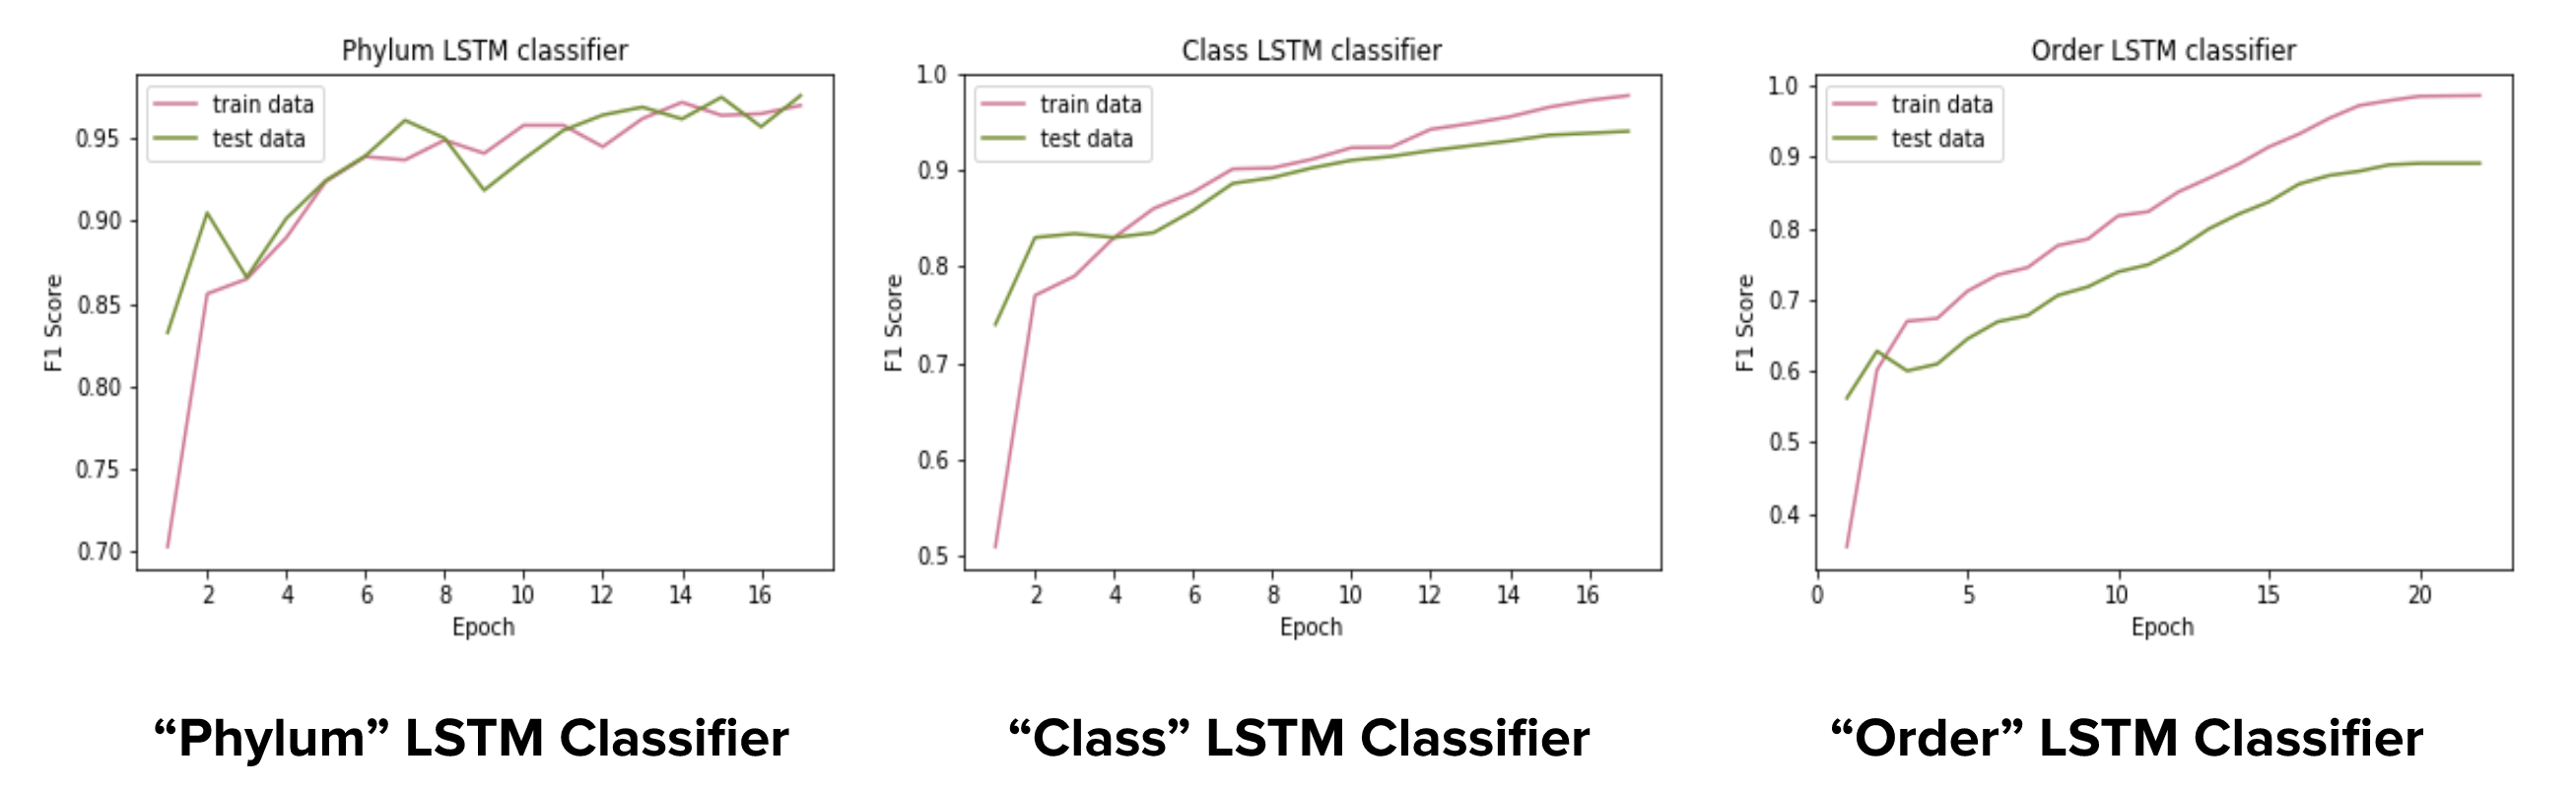
\includegraphics[scale=0.35]{lstm.png}
        \caption{F1 Score Vs. Epochs Plot: LSTM Classsifier}
        \label{fig:lstm}
        \end{figure}

\vspace*{-10mm}

\section{Significant Changes from Proposal}
\begin{enumerate}
    \item In the proposal, we filtered the DNA sequences of lengths between 1270 and 1370 and decided to use a dataset with 330K samples. But we realized that the dataset has a lot of duplicate sequences. We also wanted a compact and representative dataset to finish model training in the given time. Hence we decided to go with a dataset with 9174 samples as described above
    \item We have decided to drop the genus level classification as many classes are heavily under-represented. We have moved the family level classification to reach goals, as we have to solve the problem differently (Ex: boosting and bagging) to alleviate the problem of class imbalance.
    \item We proposed a multi-category classification approach, but we are solving three separate classification problems due to the reasons mentioned above.
\end{enumerate}

\section{Issues}
We foresee a few issues in this project which are enlisted below:
\begin{enumerate}
    \item Class imbalance at the family and genus level.
    \item Sequences are of a varied length which might be a challenge for CNN and RNN approaches. We are currently planning to truncate/pad to obtain sequences of fixed length, though there are ways to handle varying length sequences using RNNs which we will try.
    \item We are also sceptical about the deep representation learning approaches to actually model the distribution of each taxonomy-level groups.
\end{enumerate}

\begin{thebibliography}{9}
    \bibitem{src_work}
    Rizzo R., Fiannaca A., La Rosa M., Urso A.
    \textit{A Deep Learning Approach to DNA Sequence Classification}.
    Computational Intelligence Methods for Bioinformatics and Biostatistics. CIBB 2015.
    \bibitem{rdp}
    Cole, J. R., Q. Wang, J. A. Fish, B. Chai et al.
    \textit{Ribosomal Database Project: data and tools for high throughput rRNA analysis}.
    Nucl. Acids Res. 42(Database issue):D633-D642 2014
\end{thebibliography}

\end{document}
